\section{Definiciones básicas de espacios de Hilbert}
\label{sec: def basicas Hilbert}

Sea $F \in \{ \IR, \IC \}$.
Nosotros vamos a trabajar con $F-$espacios vectoriales
$V$ en los que se haya definido un \textbf{producto punto;}
si uno tiene definida una función
de este tipo (que introducimos a continuación)
es posible ya no sólo sumar y escalar elementos de $V$, sino
también hablar de \textbf{ángulos}
y \textbf{distancias} entre puntos del espacio.

\marginnote{Si $z = a + ib \in \IC$, al \textbf{conjugado
complejo} de $z$, o sea, al complejo $a-ib$, se le denota
por $\overline{z}$.}

\begin{defi}
\label{def: prod punto}
Sea $V$ un $F-$espacio vectorial. A una función
$\langle \cdot, \cdot \rangle : V \times V \longrightarrow F$
tal que, para cualesquiera $x, y, z \in V$ 
y $a, b \in F$
se cumple que 

	\begin{itemize}
	\item $\langle a \cdot x + b \cdot y, z \rangle = 
	a \langle x, z \rangle + b \langle y, z \rangle$
	\item $\langle x, y \rangle = \overline{\langle y, x \rangle} $
	\item $\langle x, x \rangle \geq 0 $
	\item $\langle x, x \rangle = 0 $ si y sólo si $x=0$
	\end{itemize}
se le llamara un \textbf{producto punto} (o \textbf{producto interior})
definido en $V$.
\end{defi}


En la sección
\ref{angulo entre elementos de un espacio con producto punto}
mostramos cómo se puede definir la noción de ángulo cuando
se cuenta con un producto punto definido en el espacio.


Observe que, según el segundo punto de la definición 
\ref{def: prod punto}, 
para todo $x \in V$ se tiene que el conjugado complejo
de $\langle x, x \rangle$ coincide con $\langle x, x \rangle$, luego
\sidenote{Por eso tiene sentido 
comparar a $\langle x, x \rangle $ con cero en el tercer punto
de la definición (no se puede definir una relación de orden en
$\IC$, c.f. \cite{marsden} p.6).},
$\langle x, x \rangle \in \IR$.

A partir de las propiedades listadas en 
\ref{def: prod punto}
que debe cumplir un 
producto punto se puede definir una norma
\sidenote{Puede consultar la definición de norma
en \cite{carothers}, p.40} en el espacio, luego, 
se tiene disponible
una noción de longitud (y, por lo tanto, de distancia también).

\begin{prop}
\label{prop: La norma inducida por un producto punto}
\textbf{(La norma inducida por un producto punto)}
Dado un espacio vectorial con
producto punto $(V, \langle \cdot , \cdot \rangle )$, 
la función $|| \cdot || : V \longrightarrow [0, \infty[$ definida como

\begin{equation}
\label{eq: norma via producto punto}
\forall v \in V: \hspace{0.2cm} || v || = \sqrt{\langle v,v \rangle}
\end{equation}

\noindent
satisface la definición de norma. A tal función se le llama
la \textbf{norma inducida por el producto punto.}
\end{prop}

Provistos de una noción de norma, siempre se puede definir
la \textbf{distancia} entre dos elementos del espacio
$x, y \in V$ como 
\begin{equation}
\label{eq: distancia a partir de norma}
d(x, y) := ||x-y||;
\end{equation}

\noindent
dotamos así a $V$ de estructura de \textbf{espacio métrico}.
\sidenote{Consulte la definición de espacio métrico en 
\cite{carothers}, p.37.}

Teniendo una estructura de espacio métrico en el espacio se 
define naturalmente una base para una \textbf{topología} en este espacio como sigue;
\begin{equation}
\label{eq: top espacio con producto punto}
\tau := \{ B_{\epsilon}(x) : \hspace{0.2cm} x \in V, \epsilon >0 \},
\end{equation}
donde 

\[
B_{\epsilon}(x) := \{ y \in V : \hspace{0.2cm} d(x,y) < \epsilon \}.
\]


\begin{figure}[H]
\centering\captionsetup{format = hang}
	\begin{measuredfigure}
		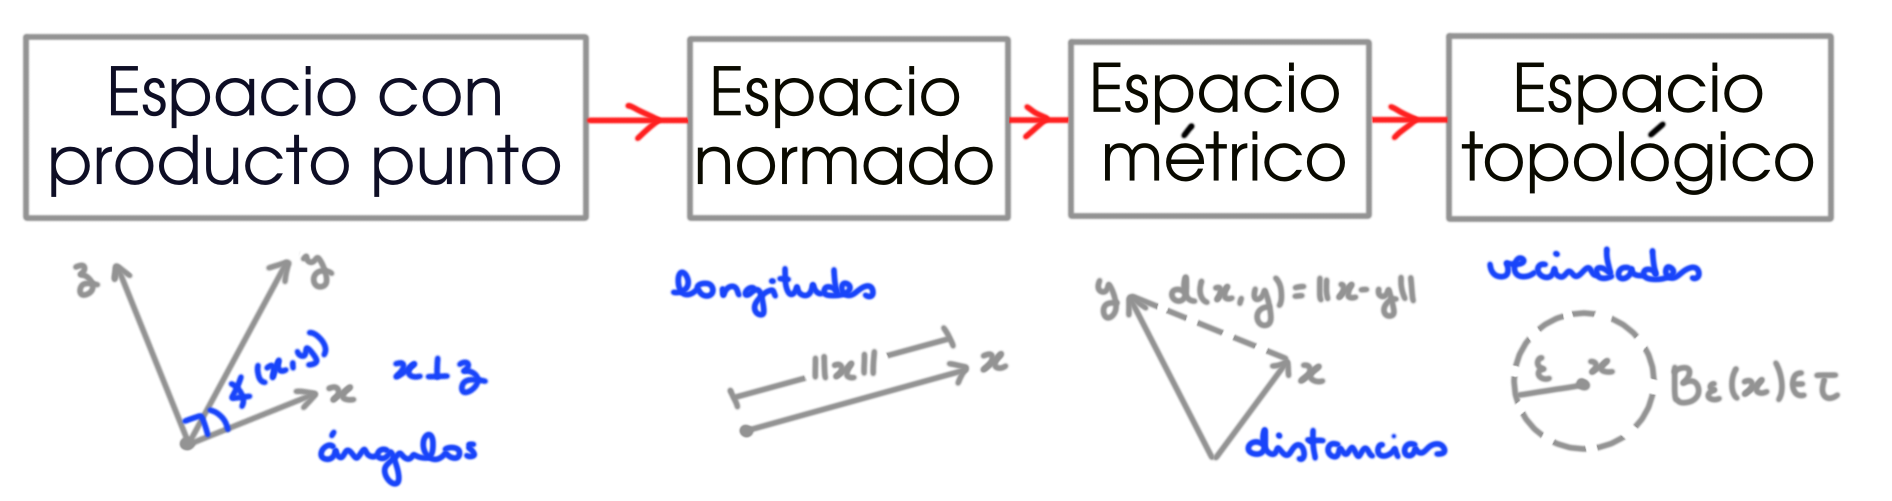
\includegraphics[scale=0.8]{estructuras} 
		\caption{El definir un producto punto en un espacio
		vectorial permite considerar en este estructuras de espacio normado,
		métrico y topológico. Se tienen pues definiciones
		matemáticas de conceptos como ``ángulo'', ``longitud'',
		``distancia'' y ``vecindad''.}
 	\end{measuredfigure}
 \end{figure}


En general, si $X$ es un conjunto no vacío y 
$d: X \times X \longrightarrow [0, \infty[$ es una función de distancia
definida en él, entonces toda \textbf{sucesión de Cauchy}
$(x_{m})_{m \in \IN}$ del espacio (es decir, toda sucesión
tal que, para todo $\epsilon >0$ sea siempre posible encontrar
un natural $N$ tal que, para cualesquiera $m, n >N$ se cumpla que
$|x_{m}-x_{n}| < \epsilon$) trivialmente converge a un punto
de $X$; 
si, recíprocamente, toda sucesión de Cauchy es convergente, 
se dice que el espacio métrico $(X, d)$ es \textbf{completo.}



\begin{defi}
\label{def: espacio de Hilbert}
Sea $(V, \langle \cdot , \cdot \rangle )$ un $F$-espacio
vectorial con producto punto. Sea $|| \cdot ||$ la norma definida como en 
\eqref{eq: norma via producto punto} y 
$d$ la distancia definida a partir de esta como en 
\eqref{eq: distancia a partir de norma}. Si el espacio
métrico $(V, d)$ es completo, entonces decimos que 
$(V, \langle \cdot , \cdot \rangle )$ es un \textbf{espacio de Hilbert.}
\end{defi}


\begin{ejemplo}
Sea $n \geq 1$.

En el $\IR-$espacio vectorial $\IR^{n}$ se tiene definido un 
producto punto canónico como sigue:

\begin{equation}
\label{eq: producto punto Rn}
\forall x=(x_{m})_{0 \leq m \leq n-1}, 
y=(y_{m})_{0 \leq m \leq n-1} \in \IR^{n}: \hspace{0.2cm}
\langle x, y \rangle = \suma{m=0}{n-1}{x_{m} y_{m}}.
\end{equation}

\noindent
En el $\IC-$espacio vectorial $\IC^{n}$ el producto canónico
se define como sigue: 


\begin{equation}
\label{eq: producto punto Cn}
\forall x=(x_{m})_{0 \leq m \leq n-1}, 
y=(y_{m})_{0 \leq m \leq n-1} \in \IC^{n}: \hspace{0.2cm}
\langle x, y \rangle = \suma{m=0}{n-1}{x_{m} \overline{y_{m}}}.
\end{equation}

Puesto que ambos espacios son finito dimensionales
(de hecho, de dimensión $n$), según \cite{mse3}
son espacios de Hilbert.
\final
\end{ejemplo}